\documentclass[aspectratio=169, 10pt]{beamer}

% --- Theme and colors ---
% Palette mirrors C_PRIMARY..C_DARK in code/evaluate.py so that the slide
% furniture and the embedded figures use one consistent scheme.
\usetheme{Madrid}
\usecolortheme{default}
\definecolor{cprimary}{HTML}{911A4B}    % burgundy   -- main model / positive class
\definecolor{csecondary}{HTML}{0D1C24}  % dark navy  -- baseline / negative class
\definecolor{ctertiary}{HTML}{5A7D8C}   % slate blue -- accents
\definecolor{cneutral}{HTML}{BBBBBB}    % light grey -- rules, de-emphasis
\definecolor{chighlight}{HTML}{A89882}  % warm taupe -- emphasis
\definecolor{cdark}{HTML}{222222}       % near-black -- text
\setbeamercolor{structure}{fg=cprimary}
\setbeamercolor{title}{fg=white, bg=cprimary}
\setbeamercolor{frametitle}{fg=white, bg=cprimary}
\setbeamercolor{block title}{fg=white, bg=cprimary}
\setbeamercolor{block body}{bg=cprimary!6}
\setbeamercolor{item}{fg=cprimary}
\setbeamercolor{alerted text}{fg=cprimary}
\setbeamercolor{section in toc}{fg=cdark}
\setbeamercolor{author in head/foot}{fg=white, bg=csecondary}
\setbeamercolor{title in head/foot}{fg=white, bg=cprimary!85!black}
\setbeamercolor{date in head/foot}{fg=white, bg=csecondary}
\setbeamertemplate{navigation symbols}{}
\setbeamertemplate{footline}{%
  \leavevmode\hbox{%
    \begin{beamercolorbox}[wd=.333\paperwidth,ht=2.5ex,dp=1ex,center]{author in head/foot}%
      \usebeamerfont{author in head/foot}\insertshortauthor
    \end{beamercolorbox}%
    \begin{beamercolorbox}[wd=.334\paperwidth,ht=2.5ex,dp=1ex,center]{title in head/foot}%
      \usebeamerfont{title in head/foot}\insertshorttitle
    \end{beamercolorbox}%
    \begin{beamercolorbox}[wd=.333\paperwidth,ht=2.5ex,dp=1ex,right]{date in head/foot}%
      \usebeamerfont{date in head/foot}\insertshortdate\hspace{2em}%
      \insertframenumber{}/\inserttotalframenumber\hspace{2ex}
    \end{beamercolorbox}}%
}

% --- Packages ---
\usepackage{amsmath,amssymb}
\usepackage{booktabs}
\usepackage{graphicx}
\usepackage{hyperref}
\usepackage{xcolor}

% --- Metadata ---
\title[Compaction Utility Prediction]{Smart Compaction:\\Predicting Compaction Utility from Lakehouse Table Metadata}
\author[Cutura \& Prakash]{%
  Jannic Alexander Cutura\textsuperscript{1,2} \and Subash Prakash\textsuperscript{3}}
\institute[ECB / DSTI / IBM]{%
  \textsuperscript{1}European Central Bank \quad
  \textsuperscript{2}DSTI School of Engineering \quad
  \textsuperscript{3}IBM}
\date{March 2026}

\begin{document}

% =============================================================
\begin{frame}
\titlepage
{\let\thefootnote\relax\footnote{\scriptsize The views expressed in this
presentation are solely those of the authors and do not necessarily reflect
the views of the European Central Bank, the European System of Central Banks
or IBM.}}
\end{frame}

% =============================================================
\begin{frame}{Outline}
\tableofcontents
\end{frame}

% =============================================================
\section{Motivation}
% =============================================================

\begin{frame}{The Small File Problem}
\begin{columns}[T]
\begin{column}{0.55\textwidth}
\textbf{Lakehouse table formats} (Iceberg, Delta Lake, Hudi):
\begin{itemize}
  \item Append-only, log-structured writes
  \item Each commit adds new immutable Parquet files
  \item Snapshot isolation + time travel
\end{itemize}
\vspace{1em}
\textbf{Consequence:} progressive file accumulation
\begin{itemize}
  \item Query planning scans every file's metadata
  \item S3 LIST/GET calls are priced per request
  \item Excessive file-open overhead degrades scans
\end{itemize}
\end{column}
\begin{column}{0.42\textwidth}
\begin{block}{At Scale}
  Catalogs with thousands of tables accumulate
  \textbf{millions} of undersized files.\\[0.5em]
  AutoComp (LinkedIn): 35,000+ Iceberg tables.
\end{block}
\vspace{0.5em}
\begin{block}{Compaction}
  Rewrites many small files $\rightarrow$ fewer target-sized files.\\[0.3em]
  But compaction \textbf{costs compute}.\\[0.3em]
  \emph{When} is it worth it?
\end{block}
\end{column}
\end{columns}
\end{frame}

% -------------------------------------------------------------

\begin{frame}{The Gap}
\begin{itemize}
  \item All open-source scheduling is \textbf{threshold-driven}:
    \begin{itemize}
      \item Iceberg: purely imperative (no built-in scheduler)
      \item Delta Lake: triggers on small-file counts
      \item Hudi: commit-count / elapsed-time rules
    \end{itemize}
  \item AutoComp (LinkedIn) uses heuristics + multi-objective Pareto
        ranking; its authors name ML prediction as future work
  \item Proprietary systems (Databricks Predictive Optimization,
        Snowflake auto-clustering, AWS S3 Tables) are
        \textbf{not open or reproducible}
  \item \textbf{No published study} examines \emph{which} metadata
        features determine compaction utility
\end{itemize}
\vspace{1em}
\begin{block}{Our Goal}
  Predict compaction utility from table metadata alone, using ML,
  and identify which features matter.
\end{block}
\end{frame}

% =============================================================
\section{Methodology}
% =============================================================

\begin{frame}{Problem Formulation}
\textbf{File count reduction ratio:}
\[
  r_{\mathrm{fc}} = 1 - \frac{n_{\mathrm{after}}}{n_{\mathrm{before}}}
\]

\vspace{0.5em}
Two tasks:
\begin{enumerate}
  \item \textbf{Classification:} Does the table need compaction?
        (did bin-packing rewrite any file, $n_{\mathrm{rewritten}} > 0$)
  \item \textbf{Regression:} Predict the continuous $r_{\mathrm{fc}} \in [0,1]$
        for cost-aware scheduling
\end{enumerate}

\vspace{1em}
\textbf{Key constraint:} features extracted only from Iceberg metadata
(manifests, snapshots, partition stats). No data files read.
\end{frame}

% -------------------------------------------------------------

\begin{frame}{Simulation Framework}
\begin{columns}[T]
\begin{column}{0.50\textwidth}
\textbf{Parameter grid:} 7 axes, 2,376 combinations
\begin{itemize}
  \item Row counts: $10^4$ to $10^6$
  \item File-size targets: 8\,KB to 128\,MB
  \item Partitions: 1 to 100
  \item Writers: 1 or 5
  \item Batches: 1 to 20
  \item Skew: uniform vs.\ Zipfian
  \item Payload: 5 or 50 UUID columns
\end{itemize}
\end{column}
\begin{column}{0.47\textwidth}
\textbf{Heterogeneous writes:}
\begin{itemize}
  \item Batch 1: 50\% of rows (initial load)
  \item Even batches: $8\times$ smaller file target
  \item Breaks the ``tautology trap''
\end{itemize}
\vspace{0.5em}
\textbf{Compaction:} Iceberg bin-packing
\begin{itemize}
  \item Target: 128\,MB
  \item Min: 96\,MB (75\%)
  \item Max: 230\,MB (180\%)
\end{itemize}
\end{column}
\end{columns}
\end{frame}

% -------------------------------------------------------------

\begin{frame}{17 Metadata Features}
\centering
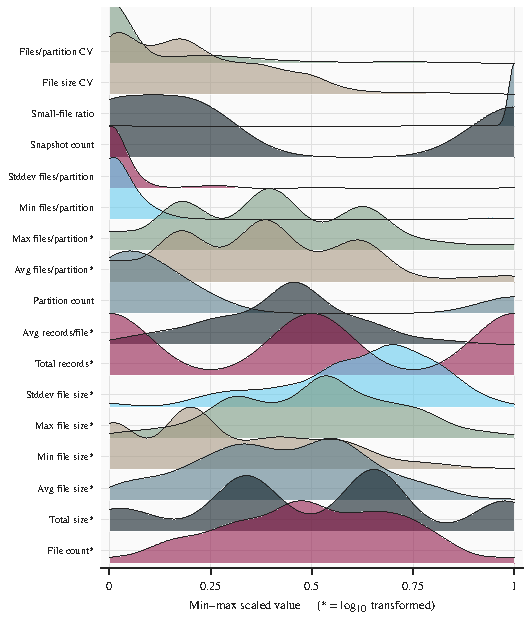
\includegraphics[height=0.76\textheight]{../paper/plots/feature_violins.pdf}\\[0.2em]
\small All 17 features, min--max scaled to $[0,1]$.
Asterisked features are $\log_{10}$-transformed.
Extracted from manifests alone --- no data file is opened.
\end{frame}

% =============================================================
\section{Results}
% =============================================================

\begin{frame}{What the Simulation Produced}
\begin{columns}[T]
\begin{column}{0.52\textwidth}
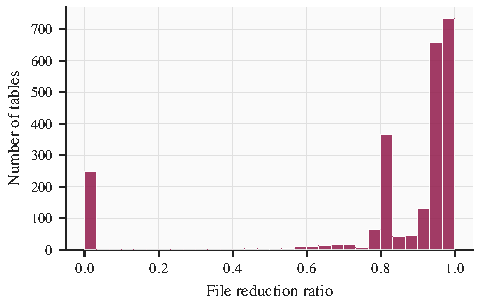
\includegraphics[width=\textwidth]{../paper/plots/label_distribution.pdf}\\[0.2em]
\small Distribution of $r_{\mathrm{fc}}$ across all 2,376 tables.
\end{column}
\begin{column}{0.46\textwidth}
\begin{itemize}
  \item \textbf{2,376} tables generated
  \item \textbf{2,121} (89.3\%) had at least one file rewritten
  \item $r_{\mathrm{fc}}$: mean 0.818, median 0.950, $\sigma = 0.294$
\end{itemize}
\vspace{0.5em}
\begin{block}{Bimodal, not continuous}
  Either compaction does essentially nothing, or it does a lot.
  Only \textbf{11 of 2,376} tables land in $(0,\,0.5]$.
\end{block}
\vspace{0.3em}
\small So the binary label and the continuous target nearly
coincide --- which is the first hint that \emph{whether} is the
easy question and \emph{how much} is the interesting one.
\end{column}
\end{columns}
\end{frame}

% -------------------------------------------------------------

\begin{frame}{Classification: Binary Decision}
\begin{columns}[T]
\begin{column}{0.48\textwidth}
\centering
\smallskip
{\small\textbf{Classification (held-out test, $n=476$)}}\\[2pt]
{\small
\begin{tabular}{lcc}
\toprule
Model & Acc. & F1 \\
\midrule
XGBoost         & 1.000 & 1.000 \\
Logistic Reg.   & 0.815 & 0.885 \\
Threshold ($k{=}4$) & 1.000 & 1.000 \\
\bottomrule
\end{tabular}}
\vspace{0.8em}
\begin{block}{The whole classifier}
  \centering\texttt{max\_files\_per\_partition}~$> 4$
\end{block}
\raggedright\small A single threshold matches XGBoost exactly.
No learned model required.
\end{column}
\begin{column}{0.50\textwidth}
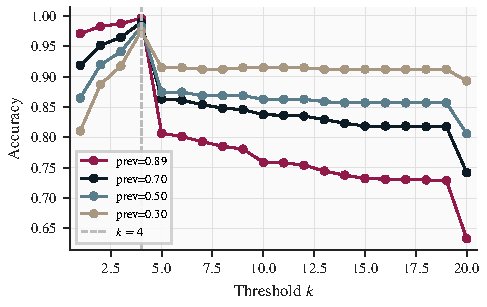
\includegraphics[width=\textwidth]{../paper/plots/threshold_prevalence.pdf}\\[0.2em]
\small Accuracy peaks at $k = 4$ and collapses at $k = 5$ ---
a hard boundary, not a fitted one. Holds at every prevalence level.
\end{column}
\end{columns}
\end{frame}

% -------------------------------------------------------------

\begin{frame}{Where the Signal Lives}
\begin{columns}[T]
\begin{column}{0.50\textwidth}
\centering
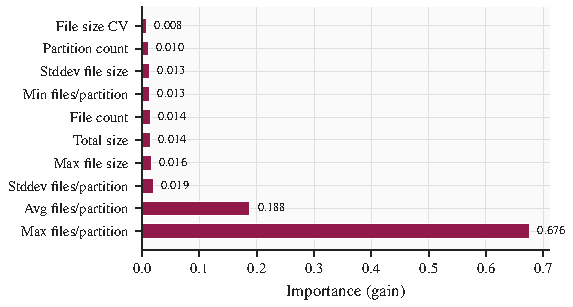
\includegraphics[width=\textwidth]{../paper/plots/feature_importance_clf.pdf}\\[0.2em]
{\small Classifier --- \textbf{86.4\%} of gain}
\end{column}
\begin{column}{0.50\textwidth}
\centering
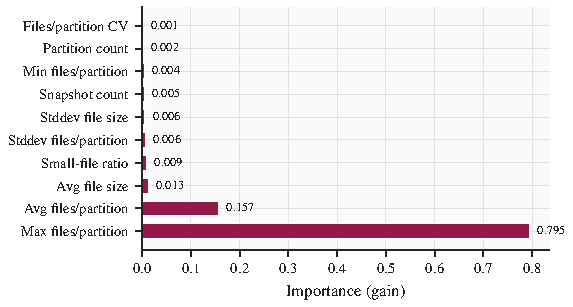
\includegraphics[width=\textwidth]{../paper/plots/feature_importance_reg.pdf}\\[0.2em]
{\small Regressor --- \textbf{95.2\%} of gain}
\end{column}
\end{columns}
\vspace{0.5em}
\centering
\small Two partition-level counts dominate both tasks.
Every other feature contributes $\leq 0.019$ gain.
\end{frame}

% -------------------------------------------------------------

\begin{frame}{Regression: Continuous Prediction}
\begin{columns}[T]
\begin{column}{0.48\textwidth}
\centering
\smallskip
{\small\textbf{Regression (held-out test)}}\\[2pt]
{\small
\begin{tabular}{lcc}
\toprule
Model & RMSE & $R^2$ \\
\midrule
XGBoost    & 0.013 & 0.998 \\
OLS        & 0.236 & 0.361 \\
\bottomrule
\end{tabular}}
\vspace{0.5em}
\begin{itemize}
  \item OLS cannot capture the nonlinear saturation curve
  \item Two features account for \textbf{95.2\%} of regressor gain
  \item Spearman $\rho = 0.965$: monotonic but not linear
\end{itemize}
\end{column}
\begin{column}{0.50\textwidth}
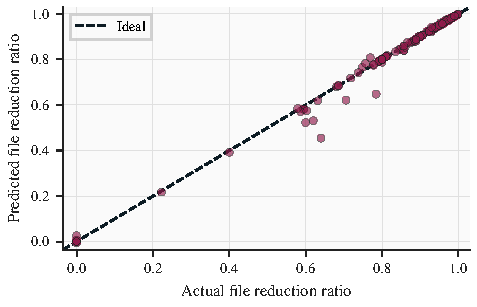
\includegraphics[width=\textwidth]{../paper/plots/regression_scatter.pdf}\\[0.2em]
\small Predicted vs.\ actual $r_{\mathrm{fc}}$ on the held-out test set.
\end{column}
\end{columns}
\end{frame}

% -------------------------------------------------------------

\begin{frame}{Is the Result Fragile?}
\begin{columns}[T]
\begin{column}{0.50\textwidth}
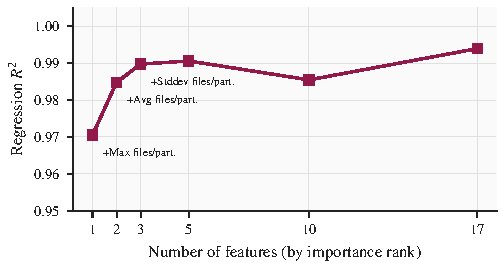
\includegraphics[width=\textwidth]{../paper/plots/feature_ablation.pdf}\\[0.2em]
\small One feature alone reaches $R^2 = 0.970$; two reach 0.985.
Past five, returns diminish.
\end{column}
\begin{column}{0.48\textwidth}
\textbf{Four robustness checks:}
\begin{itemize}
  \item \textbf{Ablation:} the other 15 features add only
        $\Delta R^2 = 0.023$ (95\% CI $[0.004, 0.044]$)
  \item \textbf{Leave-one-out:} every single removal still
        keeps $R^2 \geq 0.988$
  \item \textbf{30 bootstrap splits:} $R^2 = 0.999$,
        CI $[0.996, 1.000]$
  \item \textbf{Prevalence 89\% $\to$ 30\%:} regression
        $R^2 > 0.995$ throughout
\end{itemize}
\vspace{0.4em}
\small Holds across model families too --- random forest 0.998,
decision tree 0.997. Any tree-based model suffices; only the
linear baseline fails.
\end{column}
\end{columns}
\end{frame}

% =============================================================
\section{Cross-Schema Generalisation}
% =============================================================

\begin{frame}{TPC-H Validation (No Retraining)}
\begin{columns}[T]
\begin{column}{0.45\textwidth}
\textbf{96 Iceberg tables} from 6 TPC-H schemas\\
(lineitem, orders, customer, part, partsupp, supplier)
\begin{itemize}
  \item Realistic data types (strings, dates, decimals)
  \item 7--16 columns per schema
  \item Scale factor $\sim$10 (468.8\,M rows, 15\,GB)
\end{itemize}
\vspace{0.5em}
\centering
\smallskip
{\small\textbf{Cross-schema results}}\\[2pt]
{\small
\begin{tabular}{lcc}
\toprule
Task & Acc./RMSE & F1/$R^2$ \\
\midrule
Clf (XGBoost)            & 0.979 & 0.987 \\
Clf (Threshold $k{=}4$)  & 0.979 & 0.987 \\
Clf (\texttt{sfr}${>}0$) & 0.833 & 0.908 \\
Clf (Majority class)     & 0.823 & 0.903 \\
Reg (XGBoost)            & 0.058 & 0.976 \\
\bottomrule
\end{tabular}}
\end{column}
\begin{column}{0.53\textwidth}
\textbf{Key findings:}
\begin{itemize}
  \item Transfers with \textbf{no retraining} --- no TPC-H
        table was seen during training
  \item XGBoost and the $k{=}4$ threshold tie at 97.9\%,
        missing the same two borderline tables
        (3 files at $\sim$50\,MB)
  \item The learned model earns its keep on the
        \emph{continuous} target ($R^2 = 0.976$),
        not the binary decision
\end{itemize}
\vspace{0.3em}
\small Weakest schemas are \texttt{customer} and \texttt{partsupp}
($R^2 \approx 0.87$), which produce tables sitting closest to the
compaction threshold.
\end{column}
\end{columns}
\end{frame}

% -------------------------------------------------------------

\begin{frame}{Does Compaction Actually Make Queries Faster?}
\begin{columns}[T]
\begin{column}{0.52\textwidth}
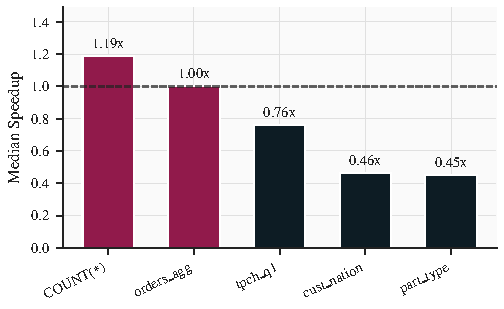
\includegraphics[width=\textwidth]{../paper/plots/query_speedup.pdf}\\[0.2em]
\small 52 TPC-H tables, Iceberg time-travel (\texttt{VERSION AS OF})
to query both snapshots. Median of 3 timed runs.
\end{column}
\begin{column}{0.46\textwidth}
\textbf{Not universally.}
\begin{itemize}
  \item \texttt{COUNT(*)}: \textbf{1.19$\times$} faster ---
        metadata overhead dominates
  \item Filtered aggregation: neutral to 0.76$\times$
  \item Full-scan aggregation: \textbf{0.45$\times$}
        --- 2$\times$ \emph{slower}
\end{itemize}
\vspace{0.5em}
\begin{block}{Why}
  Spark assigns tasks per file. Compacting 300 files into 1
  drops parallelism from 300 tasks to 1, offsetting the
  metadata saving for queries that must read everything.
\end{block}
\vspace{0.3em}
\small Overall median across 104 measurements: \textbf{0.97$\times$}.
\end{column}
\end{columns}
\end{frame}

% =============================================================
\section{Discussion}
% =============================================================

\begin{frame}{Key Insights}
\begin{block}{Tautology Trap}
  Our first grid produced only small files (max ${\sim}0.4$\,MB vs.\ the
  96\,MB threshold), so \emph{every} table compacted completely:
  $r_{\mathrm{fc}} = 1 - 1/N$. XGBoost scored $R^2 = 0.99$ by
  recovering that identity ($\rho = 0.996$). Any benchmark using
  only small synthetic files will produce misleadingly perfect metrics.
\end{block}

\vspace{0.5em}
\begin{block}{Feature Dominance}
  Partition-level file counts (\texttt{max\_files\_per\_partition},
  \texttt{avg\_files\_per\_partition}) dominate both tasks.
  \begin{itemize}
    \item Binary decision: fully solvable by a single threshold
    \item Continuous prediction: requires nonlinear modelling
  \end{itemize}
\end{block}

\vspace{0.5em}
\begin{block}{Practical Implication}
  AutoComp's compaction traits already include these features.
  They are sufficient for the binary decision --- but
  \textbf{cost-aware scheduling} needs the continuous
  prediction. A workable rule: compact when predicted
  $r_{\mathrm{fc}} > 0.3$, which drops the lowest-utility jobs
  while keeping 99.8\% of the beneficial ones.
\end{block}
\end{frame}

% -------------------------------------------------------------

\begin{frame}{Threats to Validity}
\begin{columns}[T]
\begin{column}{0.48\textwidth}
\textbf{Setup:}
\begin{itemize}
  \item Synthetic UUID payloads compress differently from real
        columnar data
  \item Partition structure generated, not domain-derived;
        query patterns not modelled
  \item Spark-local execution $\neq$ distributed clusters
        with S3
  \item 89.3\% prevalence may inflate accuracy --- mitigated by
        majority-class baseline, downsampling, bootstrap CIs
\end{itemize}
\end{column}
\begin{column}{0.48\textwidth}
\textbf{Scope --- what we did \emph{not} test:}
\begin{itemize}
  \item \textbf{Delete files / MoR:} we use Copy-on-Write only.
        Merging delete files is a different dynamic our features
        do not capture
  \item \textbf{Sort and z-order:} bin-packing only. Their utility
        depends on query workload, which metadata cannot see
  \item \textbf{Temporal evolution:} static snapshots; a table
        that is fine now may need compaction after the next write
  \item \textbf{One compaction target:} $k{=}4$ is tied to the
        128\,MB/96\,MB configuration
\end{itemize}
\end{column}
\end{columns}
\end{frame}

% =============================================================
\section{Conclusion \& Future Work}
% =============================================================

\begin{frame}{Conclusion}
\begin{enumerate}
  \item \textbf{Binary compaction decision} is trivially solvable
        by a single partition-level threshold
  \item \textbf{Continuous reduction ratio} requires nonlinear modelling\\
        (XGBoost $R^2 = 0.998$ vs.\ OLS $R^2 = 0.361$)
  \item \textbf{Transfers across schemas} without retraining:
        97.9\% on TPC-H (threshold and XGBoost alike),
        regression $R^2 = 0.976$
  \item Compaction utility is determined by \textbf{structural metadata},
        not data content
  \item Downstream benefit is \textbf{workload-dependent}: metadata-heavy
        queries speed up, full-scan aggregations slow down
\end{enumerate}

\vspace{1em}
\textbf{Future work:}
\begin{itemize}
  \item Extend to Delta Lake and Hudi
  \item Add query-workload features and cloud-cost metrics
  \item Multi-table scheduling via contextual bandits
  \item Sort and z-order compaction strategies
  \item Validation on production Iceberg catalogs
\end{itemize}

\vspace{0.5em}
\centering
\textbf{All code and data publicly available.}
\end{frame}

% =============================================================
\begin{frame}{}
\centering
\vspace{2em}
{\Large\textbf{Thank You}}\\[1.5em]
{\large Questions?}\\[2em]
\small
Jannic Alexander Cutura \quad\textbar\quad Subash Prakash\\[0.3em]
\texttt{jannic.cutura@dsti.institute} \quad\textbar\quad
\texttt{subash.prakash@ibm.com}
\end{frame}

% =============================================================
% Backup slides
% =============================================================
\appendix

\begin{frame}{Backup: Per-Schema TPC-H Breakdown}
\centering
\small
\begin{tabular}{lccc}
\toprule
Schema & $n$ & Clf Acc. & Reg $R^2$ \\
\midrule
lineitem & 16 & 1.000 & 0.997 \\
orders   & 16 & 1.000 & 1.000 \\
part     & 16 & 1.000 & 1.000 \\
supplier & 16 & 1.000 & 1.000 \\
customer & 16 & 0.938 & 0.874 \\
partsupp & 16 & 0.938 & 0.867 \\
\bottomrule
\end{tabular}
\vspace{1em}

\raggedright\small
\texttt{customer} and \texttt{partsupp} each contribute one
misclassified table. Both sit near the 96\,MB compaction
threshold, where a small file-size shift flips the outcome.
\end{frame}

% -------------------------------------------------------------

\begin{frame}{Backup: Query Latency by Type}
\centering
\small
\begin{tabular}{lccccc}
\toprule
Query & $n$ & Median & Mean & $\rho$ & $p$ \\
\midrule
\texttt{count\_star}  & 52 & 1.19$\times$ & 1.31$\times$ & 0.50 & $<$0.001 \\
\texttt{orders\_agg}  & 12 & 1.00$\times$ & 1.63$\times$ & 0.89 & $<$0.001 \\
\texttt{tpch\_q1}     & 13 & 0.76$\times$ & 0.82$\times$ & 0.77 & 0.002 \\
\texttt{cust\_nation} & 15 & 0.46$\times$ & 0.56$\times$ & 0.45 & 0.095 \\
\texttt{part\_type}   & 12 & 0.45$\times$ & 0.47$\times$ & 0.38 & 0.226 \\
\bottomrule
\end{tabular}
\vspace{1em}

\raggedright\small
52 TPC-H tables, median of 3 timed runs after 1 warmup.
Speedup $> 1\times$ means faster after compaction.
$\rho$ is the Spearman correlation with the file-reduction ratio.
\end{frame}

\end{document}
